\section{Parallélisation}

Notre code est intrinsèquement divisé en deux étape,
la première étant l'initialisation du dictionnaire,
la seconde est le calcul matriciel qui permet de
converger vers un résultat.

L'initialisation est la partie qui prend le moins
de temps à l'exécution,
phénomène d'autant plus remarquable si la taille des
documents et leur nombre augmente.
Nous avons de plus remarqué qu'il était compliqué de répartir
cette initialisation sur plusieurs noeuds MPI sans
engendrer une graphe de communication très chargé.
En effet les identifiants associés à un document
ou à un mot sont créés si ce mot/documents est relevé
pour la première fois dans l'initialisation.
Par exemple on aura alors le cas où deux noeuds
découvrent à des instants différents dans leur processus
de création de dictionnaire un document.
Ce document aura donc un identifiant i sur
le premier noeud et un identifiant j dans le second
or nous devons avoir un identifiant unique pour
un élément du dictionnaire.

Nous nous sommes donc concentrés sur la parallélisation
du calcul matriciel.
Une fois le dictionnaire et son indexation inversée
établis nous savons que les matrices de fréquence qui les
représentent ne seront plus modifiées au cours de l'algorithme.
Ainsi nous avons décidé de distribuer à chacun des sites
ces deux matrices ({\it Docs} et {\it Words}).
Notre algorithme consiste à chaque étape à comparer
les documents/mots deux à deux.
Afin que la charge de travail entre processus MPI soit
équilibrée chaque processus devra effectuer

\[ \frac{N_d \times (N_d+1)}{P \times 2}
 + \frac{N_w \times (N_w+1)}{P \times 2} \]

comparaisons à chaque étape
(avec $N_d$ le nombre total de documents,
$N_w$ le nombre total de mots et
$P$ le nombre de processus).

\begin{figure}[h]
\begin{center}
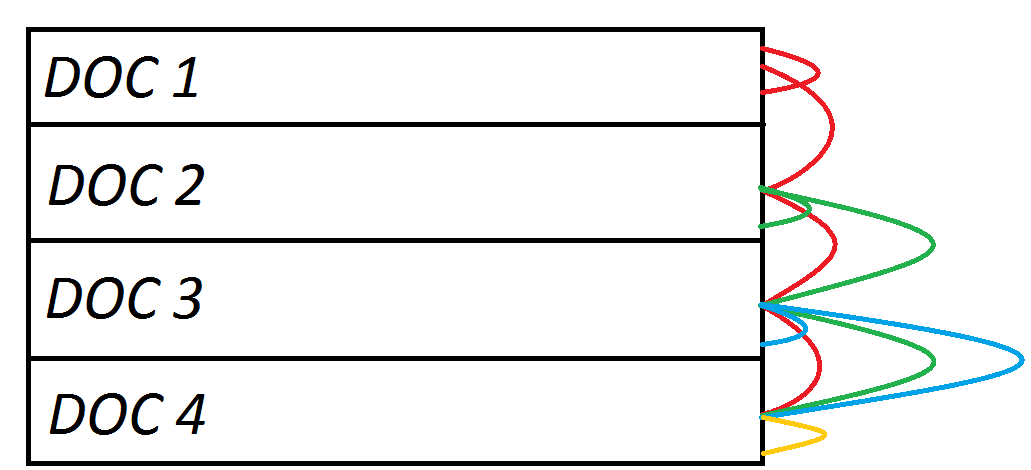
\includegraphics[height=1.5in]{cr/1}
\caption{Opérations inter-documents}
\end{center}
\end{figure}

Pour être plus précis: \newline

le processus 1 compare le document 1 avec les documents 1,2,3 et 4\newline
le processus 2 compare le document 2 avec les documents 2,3 et 4\newline
le processus 3 compare le document 2 avec les documents 3 et 4\newline
le processus 4 compare le document 2 avec les documents 4.

\newpage 
Nous obtenons donc le graphe suivant: 
 
\begin{figure}[h]
\begin{center}
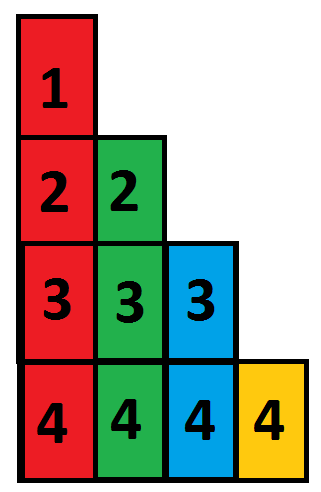
\includegraphics[height=1.5in]{cr/2}
\caption{Charge déséquilibré}
\end{center}
\end{figure}

On remarque que dans notre exemple ci-dessus, si nous souhaitons le répartir sur quatres processus MPI de façon naïf, la charge 
de travail ne sera pas  équilibré (rapport de 4 entre le processus 1 et le dernier). Il convient de répartir plus intéligement commes dans l'exemple suivant où 
il y a 10 documents, cela représente 55 combinaisons possible de comparaison. Ainsi nos 5 processus devront traiter exactement 11 combinaisons.

\begin{figure}[h]
\begin{center}
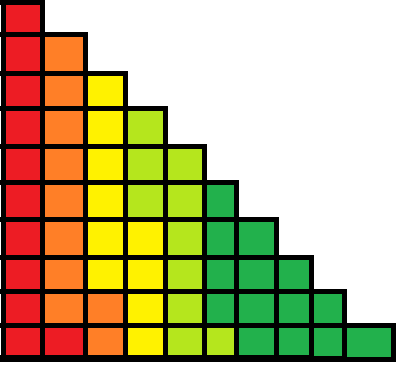
\includegraphics[height=1.5in]{cr/4}
\caption{Charge équilibré}
\end{center}
\end{figure}


Une étape est constitué des deux appels de fonctions suivant :

\begin{verbatim}
Matrix_Docs  = dist_polia(Docs, Matrix_Words)
Matrix_Words = dist_polia(Words, Matrix_Docs)
\end{verbatim}

Ici la fonction calcul une nouvealle matrice de distance à partir du matrice de fréquence et la matrice de distance complémentaire.
Les processus savent donc sur quelle plage de donnée
ils effectuent leurs calculs.
Une étape consiste à recalculer les matrices de distances
{\tt Matrix\_Docs} et {\tt Matrix\_Words}.
Ainsi entre deux appels de la fonction {\tt dist\_polia}
chaque processus doit recevoir les nouvelles distances que
les processus restant viennent de calculer.
